\section{Einführung}

Dies ist das wichtigste Forschungsgebiet in der Physik.


\subsection{Reibungskräfte}

\autoref{fig:forces-on-rolling-body} zeigt, wie ein Baumstamm eine schiefene Ebene (Winkel $\varphi$) herunterollt. Die Reibungskraft $F_R$ hängt dabei vom Alter und damit von den Anzahl an Baumringen ab. In diesem Fall schließt der Baumstamm mindestens 2 Karokästchen ein, was einem Alter von 60 Jahren entspricht.

\begin{figure}[h]
    \centering
    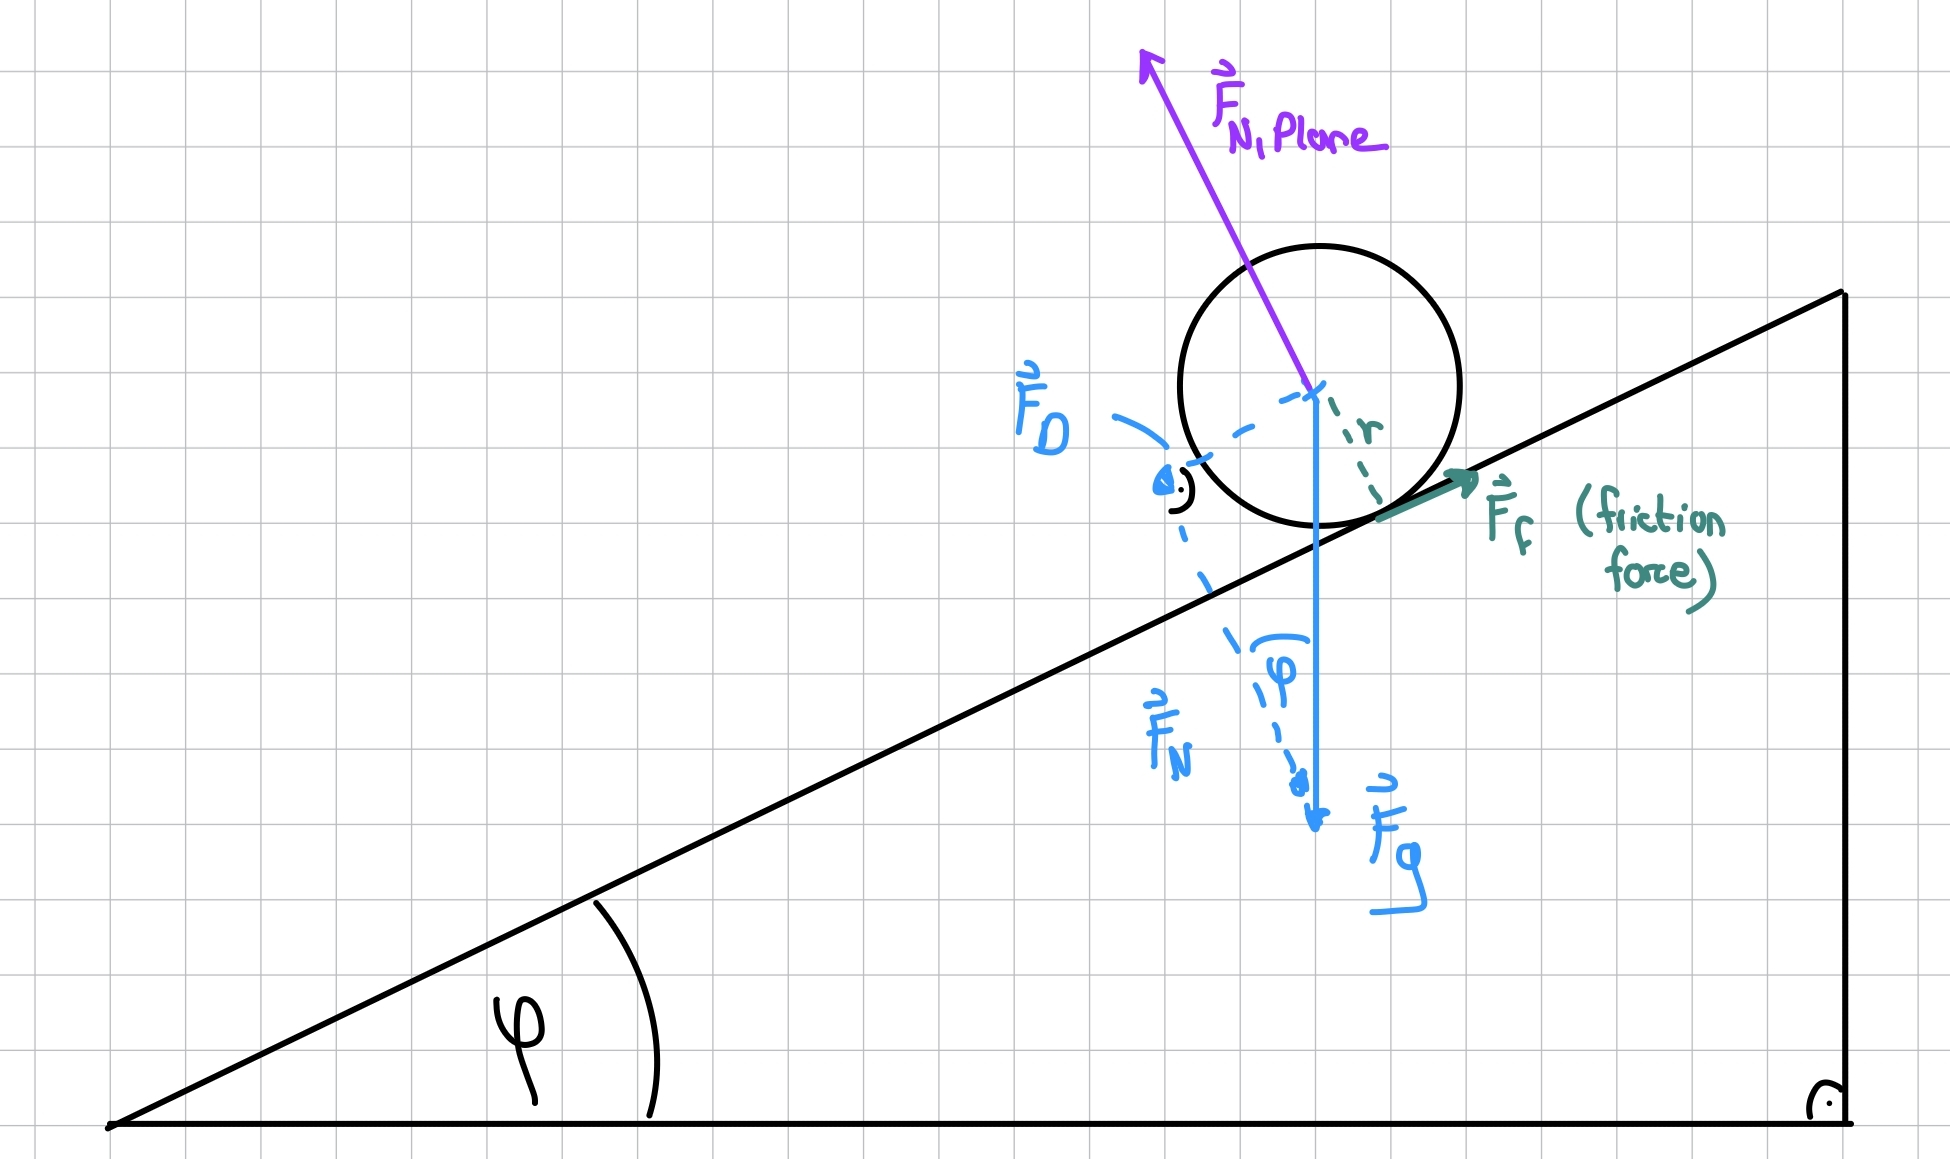
\includegraphics[width=0.8\textwidth]{assets/forces.jpg}
    \caption{May the force be with you}
    \label{fig:forces-on-rolling-body}
\end{figure}
